\documentclass{article} % For LaTeX2e
\usepackage{iclr2023_conference, times}

% --- Default packages --- 
% Optional math commands from https://github.com/goodfeli/dlbook_notation.
%%%%% NEW MATH DEFINITIONS %%%%%

\usepackage{amsmath,amsfonts,bm}

% Mark sections of captions for referring to divisions of figures
\newcommand{\figleft}{{\em (Left)}}
\newcommand{\figcenter}{{\em (Center)}}
\newcommand{\figright}{{\em (Right)}}
\newcommand{\figtop}{{\em (Top)}}
\newcommand{\figbottom}{{\em (Bottom)}}
\newcommand{\captiona}{{\em (a)}}
\newcommand{\captionb}{{\em (b)}}
\newcommand{\captionc}{{\em (c)}}
\newcommand{\captiond}{{\em (d)}}

% Highlight a newly defined term
\newcommand{\newterm}[1]{{\bf #1}}


% Figure reference, lower-case.
\def\figref#1{figure~\ref{#1}}
% Figure reference, capital. For start of sentence
\def\Figref#1{Figure~\ref{#1}}
\def\twofigref#1#2{figures \ref{#1} and \ref{#2}}
\def\quadfigref#1#2#3#4{figures \ref{#1}, \ref{#2}, \ref{#3} and \ref{#4}}
% Section reference, lower-case.
\def\secref#1{section~\ref{#1}}
% Section reference, capital.
\def\Secref#1{Section~\ref{#1}}
% Reference to two sections.
\def\twosecrefs#1#2{sections \ref{#1} and \ref{#2}}
% Reference to three sections.
\def\secrefs#1#2#3{sections \ref{#1}, \ref{#2} and \ref{#3}}
% Reference to an equation, lower-case.
\def\eqref#1{equation~\ref{#1}}
% Reference to an equation, upper case
\def\Eqref#1{Equation~\ref{#1}}
% A raw reference to an equation---avoid using if possible
\def\plaineqref#1{\ref{#1}}
% Reference to a chapter, lower-case.
\def\chapref#1{chapter~\ref{#1}}
% Reference to an equation, upper case.
\def\Chapref#1{Chapter~\ref{#1}}
% Reference to a range of chapters
\def\rangechapref#1#2{chapters\ref{#1}--\ref{#2}}
% Reference to an algorithm, lower-case.
\def\algref#1{algorithm~\ref{#1}}
% Reference to an algorithm, upper case.
\def\Algref#1{Algorithm~\ref{#1}}
\def\twoalgref#1#2{algorithms \ref{#1} and \ref{#2}}
\def\Twoalgref#1#2{Algorithms \ref{#1} and \ref{#2}}
% Reference to a part, lower case
\def\partref#1{part~\ref{#1}}
% Reference to a part, upper case
\def\Partref#1{Part~\ref{#1}}
\def\twopartref#1#2{parts \ref{#1} and \ref{#2}}

\def\ceil#1{\lceil #1 \rceil}
\def\floor#1{\lfloor #1 \rfloor}
\def\1{\bm{1}}
\newcommand{\train}{\mathcal{D}}
\newcommand{\valid}{\mathcal{D_{\mathrm{valid}}}}
\newcommand{\test}{\mathcal{D_{\mathrm{test}}}}

\def\eps{{\epsilon}}


% Random variables
\def\reta{{\textnormal{$\eta$}}}
\def\ra{{\textnormal{a}}}
\def\rb{{\textnormal{b}}}
\def\rc{{\textnormal{c}}}
\def\rd{{\textnormal{d}}}
\def\re{{\textnormal{e}}}
\def\rf{{\textnormal{f}}}
\def\rg{{\textnormal{g}}}
\def\rh{{\textnormal{h}}}
\def\ri{{\textnormal{i}}}
\def\rj{{\textnormal{j}}}
\def\rk{{\textnormal{k}}}
\def\rl{{\textnormal{l}}}
% rm is already a command, just don't name any random variables m
\def\rn{{\textnormal{n}}}
\def\ro{{\textnormal{o}}}
\def\rp{{\textnormal{p}}}
\def\rq{{\textnormal{q}}}
\def\rr{{\textnormal{r}}}
\def\rs{{\textnormal{s}}}
\def\rt{{\textnormal{t}}}
\def\ru{{\textnormal{u}}}
\def\rv{{\textnormal{v}}}
\def\rw{{\textnormal{w}}}
\def\rx{{\textnormal{x}}}
\def\ry{{\textnormal{y}}}
\def\rz{{\textnormal{z}}}

% Random vectors
\def\rvepsilon{{\mathbf{\epsilon}}}
\def\rvtheta{{\mathbf{\theta}}}
\def\rva{{\mathbf{a}}}
\def\rvb{{\mathbf{b}}}
\def\rvc{{\mathbf{c}}}
\def\rvd{{\mathbf{d}}}
\def\rve{{\mathbf{e}}}
\def\rvf{{\mathbf{f}}}
\def\rvg{{\mathbf{g}}}
\def\rvh{{\mathbf{h}}}
\def\rvu{{\mathbf{i}}}
\def\rvj{{\mathbf{j}}}
\def\rvk{{\mathbf{k}}}
\def\rvl{{\mathbf{l}}}
\def\rvm{{\mathbf{m}}}
\def\rvn{{\mathbf{n}}}
\def\rvo{{\mathbf{o}}}
\def\rvp{{\mathbf{p}}}
\def\rvq{{\mathbf{q}}}
\def\rvr{{\mathbf{r}}}
\def\rvs{{\mathbf{s}}}
\def\rvt{{\mathbf{t}}}
\def\rvu{{\mathbf{u}}}
\def\rvv{{\mathbf{v}}}
\def\rvw{{\mathbf{w}}}
\def\rvx{{\mathbf{x}}}
\def\rvy{{\mathbf{y}}}
\def\rvz{{\mathbf{z}}}

% Elements of random vectors
\def\erva{{\textnormal{a}}}
\def\ervb{{\textnormal{b}}}
\def\ervc{{\textnormal{c}}}
\def\ervd{{\textnormal{d}}}
\def\erve{{\textnormal{e}}}
\def\ervf{{\textnormal{f}}}
\def\ervg{{\textnormal{g}}}
\def\ervh{{\textnormal{h}}}
\def\ervi{{\textnormal{i}}}
\def\ervj{{\textnormal{j}}}
\def\ervk{{\textnormal{k}}}
\def\ervl{{\textnormal{l}}}
\def\ervm{{\textnormal{m}}}
\def\ervn{{\textnormal{n}}}
\def\ervo{{\textnormal{o}}}
\def\ervp{{\textnormal{p}}}
\def\ervq{{\textnormal{q}}}
\def\ervr{{\textnormal{r}}}
\def\ervs{{\textnormal{s}}}
\def\ervt{{\textnormal{t}}}
\def\ervu{{\textnormal{u}}}
\def\ervv{{\textnormal{v}}}
\def\ervw{{\textnormal{w}}}
\def\ervx{{\textnormal{x}}}
\def\ervy{{\textnormal{y}}}
\def\ervz{{\textnormal{z}}}

% Random matrices
\def\rmA{{\mathbf{A}}}
\def\rmB{{\mathbf{B}}}
\def\rmC{{\mathbf{C}}}
\def\rmD{{\mathbf{D}}}
\def\rmE{{\mathbf{E}}}
\def\rmF{{\mathbf{F}}}
\def\rmG{{\mathbf{G}}}
\def\rmH{{\mathbf{H}}}
\def\rmI{{\mathbf{I}}}
\def\rmJ{{\mathbf{J}}}
\def\rmK{{\mathbf{K}}}
\def\rmL{{\mathbf{L}}}
\def\rmM{{\mathbf{M}}}
\def\rmN{{\mathbf{N}}}
\def\rmO{{\mathbf{O}}}
\def\rmP{{\mathbf{P}}}
\def\rmQ{{\mathbf{Q}}}
\def\rmR{{\mathbf{R}}}
\def\rmS{{\mathbf{S}}}
\def\rmT{{\mathbf{T}}}
\def\rmU{{\mathbf{U}}}
\def\rmV{{\mathbf{V}}}
\def\rmW{{\mathbf{W}}}
\def\rmX{{\mathbf{X}}}
\def\rmY{{\mathbf{Y}}}
\def\rmZ{{\mathbf{Z}}}

% Elements of random matrices
\def\ermA{{\textnormal{A}}}
\def\ermB{{\textnormal{B}}}
\def\ermC{{\textnormal{C}}}
\def\ermD{{\textnormal{D}}}
\def\ermE{{\textnormal{E}}}
\def\ermF{{\textnormal{F}}}
\def\ermG{{\textnormal{G}}}
\def\ermH{{\textnormal{H}}}
\def\ermI{{\textnormal{I}}}
\def\ermJ{{\textnormal{J}}}
\def\ermK{{\textnormal{K}}}
\def\ermL{{\textnormal{L}}}
\def\ermM{{\textnormal{M}}}
\def\ermN{{\textnormal{N}}}
\def\ermO{{\textnormal{O}}}
\def\ermP{{\textnormal{P}}}
\def\ermQ{{\textnormal{Q}}}
\def\ermR{{\textnormal{R}}}
\def\ermS{{\textnormal{S}}}
\def\ermT{{\textnormal{T}}}
\def\ermU{{\textnormal{U}}}
\def\ermV{{\textnormal{V}}}
\def\ermW{{\textnormal{W}}}
\def\ermX{{\textnormal{X}}}
\def\ermY{{\textnormal{Y}}}
\def\ermZ{{\textnormal{Z}}}

% Vectors
\def\vzero{{\bm{0}}}
\def\vone{{\bm{1}}}
\def\vmu{{\bm{\mu}}}
\def\vtheta{{\bm{\theta}}}
\def\va{{\bm{a}}}
\def\vb{{\bm{b}}}
\def\vc{{\bm{c}}}
\def\vd{{\bm{d}}}
\def\ve{{\bm{e}}}
\def\vf{{\bm{f}}}
\def\vg{{\bm{g}}}
\def\vh{{\bm{h}}}
\def\vi{{\bm{i}}}
\def\vj{{\bm{j}}}
\def\vk{{\bm{k}}}
\def\vl{{\bm{l}}}
\def\vm{{\bm{m}}}
\def\vn{{\bm{n}}}
\def\vo{{\bm{o}}}
\def\vp{{\bm{p}}}
\def\vq{{\bm{q}}}
\def\vr{{\bm{r}}}
\def\vs{{\bm{s}}}
\def\vt{{\bm{t}}}
\def\vu{{\bm{u}}}
\def\vv{{\bm{v}}}
\def\vw{{\bm{w}}}
\def\vx{{\bm{x}}}
\def\vy{{\bm{y}}}
\def\vz{{\bm{z}}}

% Elements of vectors
\def\evalpha{{\alpha}}
\def\evbeta{{\beta}}
\def\evepsilon{{\epsilon}}
\def\evlambda{{\lambda}}
\def\evomega{{\omega}}
\def\evmu{{\mu}}
\def\evpsi{{\psi}}
\def\evsigma{{\sigma}}
\def\evtheta{{\theta}}
\def\eva{{a}}
\def\evb{{b}}
\def\evc{{c}}
\def\evd{{d}}
\def\eve{{e}}
\def\evf{{f}}
\def\evg{{g}}
\def\evh{{h}}
\def\evi{{i}}
\def\evj{{j}}
\def\evk{{k}}
\def\evl{{l}}
\def\evm{{m}}
\def\evn{{n}}
\def\evo{{o}}
\def\evp{{p}}
\def\evq{{q}}
\def\evr{{r}}
\def\evs{{s}}
\def\evt{{t}}
\def\evu{{u}}
\def\evv{{v}}
\def\evw{{w}}
\def\evx{{x}}
\def\evy{{y}}
\def\evz{{z}}

% Matrix
\def\mA{{\bm{A}}}
\def\mB{{\bm{B}}}
\def\mC{{\bm{C}}}
\def\mD{{\bm{D}}}
\def\mE{{\bm{E}}}
\def\mF{{\bm{F}}}
\def\mG{{\bm{G}}}
\def\mH{{\bm{H}}}
\def\mI{{\bm{I}}}
\def\mJ{{\bm{J}}}
\def\mK{{\bm{K}}}
\def\mL{{\bm{L}}}
\def\mM{{\bm{M}}}
\def\mN{{\bm{N}}}
\def\mO{{\bm{O}}}
\def\mP{{\bm{P}}}
\def\mQ{{\bm{Q}}}
\def\mR{{\bm{R}}}
\def\mS{{\bm{S}}}
\def\mT{{\bm{T}}}
\def\mU{{\bm{U}}}
\def\mV{{\bm{V}}}
\def\mW{{\bm{W}}}
\def\mX{{\bm{X}}}
\def\mY{{\bm{Y}}}
\def\mZ{{\bm{Z}}}
\def\mBeta{{\bm{\beta}}}
\def\mPhi{{\bm{\Phi}}}
\def\mLambda{{\bm{\Lambda}}}
\def\mSigma{{\bm{\Sigma}}}

% Tensor
\DeclareMathAlphabet{\mathsfit}{\encodingdefault}{\sfdefault}{m}{sl}
\SetMathAlphabet{\mathsfit}{bold}{\encodingdefault}{\sfdefault}{bx}{n}
\newcommand{\tens}[1]{\bm{\mathsfit{#1}}}
\def\tA{{\tens{A}}}
\def\tB{{\tens{B}}}
\def\tC{{\tens{C}}}
\def\tD{{\tens{D}}}
\def\tE{{\tens{E}}}
\def\tF{{\tens{F}}}
\def\tG{{\tens{G}}}
\def\tH{{\tens{H}}}
\def\tI{{\tens{I}}}
\def\tJ{{\tens{J}}}
\def\tK{{\tens{K}}}
\def\tL{{\tens{L}}}
\def\tM{{\tens{M}}}
\def\tN{{\tens{N}}}
\def\tO{{\tens{O}}}
\def\tP{{\tens{P}}}
\def\tQ{{\tens{Q}}}
\def\tR{{\tens{R}}}
\def\tS{{\tens{S}}}
\def\tT{{\tens{T}}}
\def\tU{{\tens{U}}}
\def\tV{{\tens{V}}}
\def\tW{{\tens{W}}}
\def\tX{{\tens{X}}}
\def\tY{{\tens{Y}}}
\def\tZ{{\tens{Z}}}


% Graph
\def\gA{{\mathcal{A}}}
\def\gB{{\mathcal{B}}}
\def\gC{{\mathcal{C}}}
\def\gD{{\mathcal{D}}}
\def\gE{{\mathcal{E}}}
\def\gF{{\mathcal{F}}}
\def\gG{{\mathcal{G}}}
\def\gH{{\mathcal{H}}}
\def\gI{{\mathcal{I}}}
\def\gJ{{\mathcal{J}}}
\def\gK{{\mathcal{K}}}
\def\gL{{\mathcal{L}}}
\def\gM{{\mathcal{M}}}
\def\gN{{\mathcal{N}}}
\def\gO{{\mathcal{O}}}
\def\gP{{\mathcal{P}}}
\def\gQ{{\mathcal{Q}}}
\def\gR{{\mathcal{R}}}
\def\gS{{\mathcal{S}}}
\def\gT{{\mathcal{T}}}
\def\gU{{\mathcal{U}}}
\def\gV{{\mathcal{V}}}
\def\gW{{\mathcal{W}}}
\def\gX{{\mathcal{X}}}
\def\gY{{\mathcal{Y}}}
\def\gZ{{\mathcal{Z}}}

% Sets
\def\sA{{\mathbb{A}}}
\def\sB{{\mathbb{B}}}
\def\sC{{\mathbb{C}}}
\def\sD{{\mathbb{D}}}
% Don't use a set called E, because this would be the same as our symbol
% for expectation.
\def\sF{{\mathbb{F}}}
\def\sG{{\mathbb{G}}}
\def\sH{{\mathbb{H}}}
\def\sI{{\mathbb{I}}}
\def\sJ{{\mathbb{J}}}
\def\sK{{\mathbb{K}}}
\def\sL{{\mathbb{L}}}
\def\sM{{\mathbb{M}}}
\def\sN{{\mathbb{N}}}
\def\sO{{\mathbb{O}}}
\def\sP{{\mathbb{P}}}
\def\sQ{{\mathbb{Q}}}
\def\sR{{\mathbb{R}}}
\def\sS{{\mathbb{S}}}
\def\sT{{\mathbb{T}}}
\def\sU{{\mathbb{U}}}
\def\sV{{\mathbb{V}}}
\def\sW{{\mathbb{W}}}
\def\sX{{\mathbb{X}}}
\def\sY{{\mathbb{Y}}}
\def\sZ{{\mathbb{Z}}}

% Entries of a matrix
\def\emLambda{{\Lambda}}
\def\emA{{A}}
\def\emB{{B}}
\def\emC{{C}}
\def\emD{{D}}
\def\emE{{E}}
\def\emF{{F}}
\def\emG{{G}}
\def\emH{{H}}
\def\emI{{I}}
\def\emJ{{J}}
\def\emK{{K}}
\def\emL{{L}}
\def\emM{{M}}
\def\emN{{N}}
\def\emO{{O}}
\def\emP{{P}}
\def\emQ{{Q}}
\def\emR{{R}}
\def\emS{{S}}
\def\emT{{T}}
\def\emU{{U}}
\def\emV{{V}}
\def\emW{{W}}
\def\emX{{X}}
\def\emY{{Y}}
\def\emZ{{Z}}
\def\emSigma{{\Sigma}}

% entries of a tensor
% Same font as tensor, without \bm wrapper
\newcommand{\etens}[1]{\mathsfit{#1}}
\def\etLambda{{\etens{\Lambda}}}
\def\etA{{\etens{A}}}
\def\etB{{\etens{B}}}
\def\etC{{\etens{C}}}
\def\etD{{\etens{D}}}
\def\etE{{\etens{E}}}
\def\etF{{\etens{F}}}
\def\etG{{\etens{G}}}
\def\etH{{\etens{H}}}
\def\etI{{\etens{I}}}
\def\etJ{{\etens{J}}}
\def\etK{{\etens{K}}}
\def\etL{{\etens{L}}}
\def\etM{{\etens{M}}}
\def\etN{{\etens{N}}}
\def\etO{{\etens{O}}}
\def\etP{{\etens{P}}}
\def\etQ{{\etens{Q}}}
\def\etR{{\etens{R}}}
\def\etS{{\etens{S}}}
\def\etT{{\etens{T}}}
\def\etU{{\etens{U}}}
\def\etV{{\etens{V}}}
\def\etW{{\etens{W}}}
\def\etX{{\etens{X}}}
\def\etY{{\etens{Y}}}
\def\etZ{{\etens{Z}}}

% The true underlying data generating distribution
\newcommand{\pdata}{p_{\rm{data}}}
% The empirical distribution defined by the training set
\newcommand{\ptrain}{\hat{p}_{\rm{data}}}
\newcommand{\Ptrain}{\hat{P}_{\rm{data}}}
% The model distribution
\newcommand{\pmodel}{p_{\rm{model}}}
\newcommand{\Pmodel}{P_{\rm{model}}}
\newcommand{\ptildemodel}{\tilde{p}_{\rm{model}}}
% Stochastic autoencoder distributions
\newcommand{\pencode}{p_{\rm{encoder}}}
\newcommand{\pdecode}{p_{\rm{decoder}}}
\newcommand{\precons}{p_{\rm{reconstruct}}}

\newcommand{\laplace}{\mathrm{Laplace}} % Laplace distribution

\newcommand{\E}{\mathbb{E}}
\newcommand{\Ls}{\mathcal{L}}
\newcommand{\R}{\mathbb{R}}
\newcommand{\emp}{\tilde{p}}
\newcommand{\lr}{\alpha}
\newcommand{\reg}{\lambda}
\newcommand{\rect}{\mathrm{rectifier}}
\newcommand{\softmax}{\mathrm{softmax}}
\newcommand{\sigmoid}{\sigma}
\newcommand{\softplus}{\zeta}
\newcommand{\KL}{D_{\mathrm{KL}}}
\newcommand{\Var}{\mathrm{Var}}
\newcommand{\standarderror}{\mathrm{SE}}
\newcommand{\Cov}{\mathrm{Cov}}
% Wolfram Mathworld says $L^2$ is for function spaces and $\ell^2$ is for vectors
% But then they seem to use $L^2$ for vectors throughout the site, and so does
% wikipedia.
\newcommand{\normlzero}{L^0}
\newcommand{\normlone}{L^1}
\newcommand{\normltwo}{L^2}
\newcommand{\normlp}{L^p}
\newcommand{\normmax}{L^\infty}

\newcommand{\parents}{Pa} % See usage in notation.tex. Chosen to match Daphne's book.

\DeclareMathOperator*{\argmax}{arg\,max}
\DeclareMathOperator*{\argmin}{arg\,min}

\DeclareMathOperator{\sign}{sign}
\DeclareMathOperator{\Tr}{Tr}
\let\ab\allowbreak

\usepackage{hyperref}
\usepackage{url}

% --- Custom packages --- 
% images
\usepackage{graphicx}
\usepackage{float}
\usepackage{wrapfig}

% psudeocode
\usepackage{algorithm}
\usepackage{algpseudocode}
\def\NoNumber#1{{\def\alglinenumber##1{}\State #1}\addtocounter{ALG@line}{-1}}

\newtheorem{theorem}{Theorem}
\newtheorem{definition}{Definition}
\newtheorem{lemma}{Lemma}

\newcommand{\indep}{\perp \!\!\! \perp}

\newcommand{\yli}[1]{{\color{cyan}#1}}

\title{
    Trusted Aggregation (TAG): Model Filtering Backdoor Defense In Federated Learning
}

% Authors must not appear in the submitted version. They should be hidden
% as long as the \iclrfinalcopy macro remains commented out below.
% Non-anonymous submissions will be rejected without review.

\author{%
    Joseph Lavond \& Yao Li  \\
    Department of Statistics and Operations Research \\
    University of North Carolina at Chapel Hill \\
    Chapel Hill, NC 27514, USA \\
    \texttt{\{jlavond, yaoli\}@unc.email.edu} \\
    %
    \And
    Minhao Cheng \\
    Computer Science and Engineering \\
    Hong Kong University of Science and Technology \\
    Clear Water Bay, Hong Kong \\
    \texttt{minhaocheng@ust.hk}
}

% The \author macro works with any number of authors. There are two commands
% used to separate the names and addresses of multiple authors: \And and \AND.
%
% Using \And between authors leaves it to \LaTeX{} to determine where to break
% the lines. Using \AND forces a linebreak at that point. So, if \LaTeX{}
% puts 3 of 4 authors names on the first line, and the last on the second
% line, try using \AND instead of \And before the third author name.

\newcommand{\fix}{\marginpar{FIX}}
\newcommand{\new}{\marginpar{NEW}}

%\iclrfinalcopy % Uncomment for camera-ready version, but NOT for submission.
\begin{document}


\maketitle

\begin{abstract}
Abstract text here.
\end{abstract}



% ----- Content -----
\section{Introduction}

Federated learning is a potential solution to constructing a machine learning model from several local data sources that cannot be exchanged or aggregated. As mentioned in \cite{fed-learn}, these restrictions are essential in areas where data privacy or security is critical, including but not limited to healthcare and defense. Additionally, federated learning is valuable for companies wishing to shift computing workload to local devices. Furthermore, these local datasets are not required to be independent and identically distributed. Hence, a shared robust global model is desirable and, in many cases, cannot be produced without some form of collaborative learning. \yli{need citations for this paragraph}


Concerns have arisen that the lack of control or knowledge regarding the local training procedure could allow a user, with malicious intent, to create an update that compromises the global model for all future users. An example of such harm is a backdoor attack, where training attempt to get a model to associate a given manipulation of the input data, known as a trigger, with a particular outcome. Recent work, such as by \cite{stamp-invisible}., creates backdoor triggers that are not detectable in the data by either human or computer vision when included within the data. However, in federated learning, only the resulting model gradients or weights are communicated back, so there is potentially no need to hide the trigger in the data. Furthermore, without access to leverage user input data, there is less information available to help detect and prevent such malicious intent. Thus backdoor attacks may be easier to perform and harder to detect in federated learning.

Our contribution to federated learning is establishing defense criteria for federated learning, which is effective against multiple attackers, model scaling, and attacks before global model convergence. Furthermore, our threshold still allows many regular users to update the global model, resulting in little to no performance degradation and requiring only a minimal increase in computational resources or time.

%
\section{Related Work}

\paragraph{Federated Learning.} At a high level, federated learning is an iterative procedure involving rounds of model improvement until it meets some criteria. These rounds first send the global model to users and select a subset of users to update the global model. Then those chosen users train their local copy of the model, and their resulting models are communicated back and aggregated to create a new global model. Typically, the final local model's gradients or weights are transmitted back to ensure data privacy.

\paragraph{Backdoor Attack \& Defense.} \cite{dba} shows that the multiple-user nature of federated learning is exploitable to make more potent and lasting backdoor attacks. By distributing the backdoor trigger across a few malicious users, they could make the global model exhibit the desired behavior at higher rates and for many iterations after the attack had concluded. We will show our threshold's effectiveness in even more potent attack settings than in their original paper.

Next, \cite{trim-mean} proposed the current state-of-the-ark defense method for federated learning. Their paper theoretically explores two robust aggregation methods of user-returned model weights. In our experiments, we will compare our proposed method to both their coordinate-wise median and trimmed-mean procedures.

\begin{definition}[Coordinate-wise median] 
For vectors $x_i \in \mathbb{R}^{d}$ for $i \in \mathopen[N\mathclose]$, the coordinate-wise median g has element k defined as follows $g^{(k)} = median(\{x_i^{(k)} \mid i \in N\})$.
\end{definition}

\begin{definition}[Coordinate-wise trimmed-mean]
For $\beta \in \mathopen[ 0, 0.5 \mathclose)$ and vectors $x_i \in \mathbb{R}^{d}$ for $i \in \mathopen[I\mathclose]$, the coordinate-wise trimmed-mean g has element k defined as:
\begin{align*}
g^{(k)} = \dfrac{\sum_{j \in J}{x_j^{(k)}}}{(1 - 2\beta)N}
\end{align*}
where $J \subseteq I$ is the collection of indices that do not include the top and bottom $\beta$ proportion of the sorted $x_i^{(k)}$ values.
\end{definition}

Currently, many defense methods are based on modifications to the aggregation method. We propose a model filtering method that can be implemented in addition to other aggregation methods or model filtering. Since our threshold can be implemented for many aggregation methods, we focus on the original FedAvg procedure, proposed by \cite{fedavg}. Under FedAvg, the aggregation step consists of setting the next iteration of the global model to the average of user-returned updated models. 


%
\section{Method}

In this section, we describe the motivation and framework for our proposed method, Trusted Aggregation (TAG), which ADVANTAGE OF THE METHOD. 

\paragraph{Motivation}

We find that the output layer distributions of malicious users are very different from that of benign users. Note that there is a discernible difference between malicious and benign user distributions for the target label class. Therefore, we can leverage this difference to detect backdoor attacks. Figure \ref{fig:motivation} shows a model with different estimated distributions for the target class depending on whether or not that model has been backdoor attacked. 

\begin{figure}[H]
    \centering
    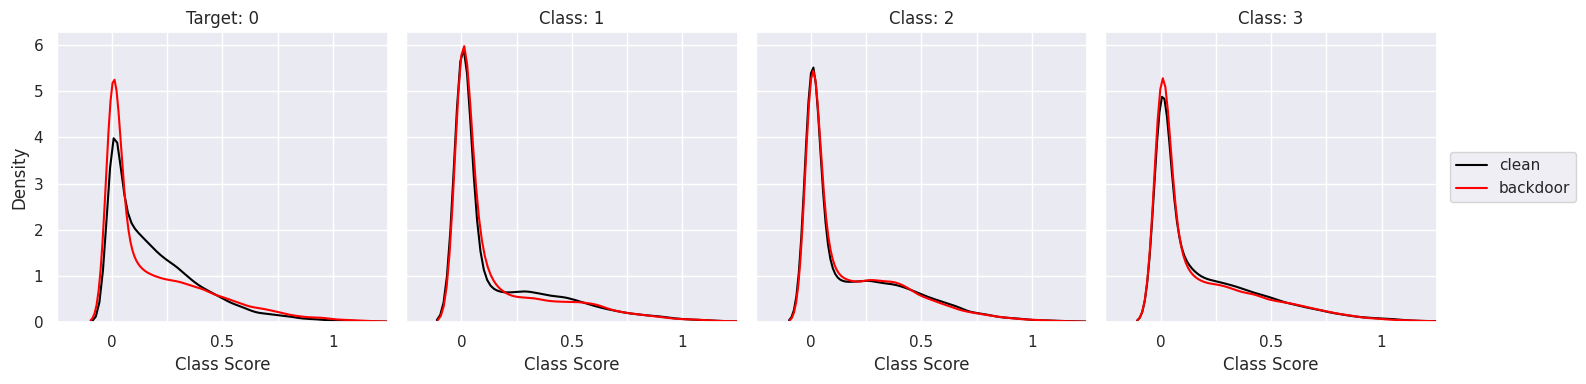
\includegraphics[width=\textwidth]{make_article/make_visuals/visuals/ext_motivation.png}
    \caption{Kernel Density Estimation from Predicted Scores}
    \label{fig:motivation}
\end{figure}

\paragraph{Detection Framework}

We assume that there exists one user who we can be confident is trustworthy to place in charge of gate-keeping the global model for updates. The detection method leverages the trusted user to evaluate incoming model weights and determine whether each contribution is allowed to participate in the global model update procedure. The main idea is to detect user models with an unusually distributed output layer with the information from a single trusted user. Moving forward, we will refer to this single trusted user as the validation user. In each communication round, this validation user completes the following additional steps to generate a threshold for malicious user detection, see Algorithm \ref{alg:t-agg}

\begin{algorithm}[H]
\caption{ (Trusted Aggregation) \\ 
Notation: Let $S$ represent the random subset of users that will submit locally trained models $U$ to update the global model $G$, $T$ to denote the trusted user, and $D$ to identify some distributional difference function.
}
\label{alg:t-agg}
\begin{algorithmic}[1]

    \Procedure{Trusted Aggregation}{G, U_T, $\{U_j \mid j \in S\}$}
        \For{each class with trusted user's data $(X, y)$}
            \State predict scores: $o_G = G(X)$, $o_{T} = U_T(X)$, and $o_j = U_j(X)$, $\forall j \in S$
            \State calculate empirical CDFs for each predicted score above 
            \State \quad and compute the distributional distances between each user and global models 
            \State \quad $v_T = D(o_G, o_T)$ and $v_{j} = D(o_G, o_{j})$, $\forall j \in S$
            \State $v_T \gets \Call{Class Frequency Scaling}{v_T}$  \Comment{(Algorithm \ref{alg:scaling})}
        \EndFor
        \State compute round threshold $c_r = 2 * \max ( \{v_T\} )$
        \State  $c_r \gets \Call{Global-Min Mean Smoothing}{c_r}$  \Comment{(Algorithm \ref{alg:smoothing})}
        \State define $S_r = \{j \in S | \max (\{v_{j}\}) < c_r \} \subseteq S$
        \State \Return FedAvg$(\{U_j \mid j \in S_T \})$ 
    \EndProcedure
\end{algorithmic}
\end{algorithm}


%
\paragraph{Threshold Construction.} Recall that we intend to determine the most considerable possible change that a non-malicious user could contribute and exclude all users from participating in the update of the global model that exceeds such a threshold. Hence, we want to estimate the most prominent possible KS distance for any class for use as a cutoff. We operate under the assumption that the class distances are Uniform on $\mathopen[0, b_c\mathclose]$ for each class c, where $b_c$ is the maximum possible change to the output layer of class c through local training by a non-malicious user. Therefore, we aim to estimate and use a representation for the maximum of $b_c$ ($U$), the maximal benign change to any class, as a cutoff for returning user models. Letting $D$ represent the total number of classes, equation \ref{eq:geq_bound} shows under our distributional assumptions that twice the maximum of the class conditional differences is, on average, a practical upper bound for accepting benign submissions.

\begin{align}
    & \textrm{Suppose } \forall c \in \mathopen[ D \mathclose], (KS)_c \sim \textrm{ Uniform}(0, b_c) \nonumber \\
    & \textrm{Let } j = \argmax_c \left( b_c \right) \textrm{ such that } b_j = \max_c \left( b_c \right) \nonumber \\
    & \quad \max_c \left( (KS)_c \right) \geq (KS)_j \nonumber \\
    & \quad E \left[ \max_c \left( (KS)_c \right) \right] \geq E \left[ (KS)_j \right] = \dfrac{b_j}{2} \nonumber \\
    & \quad E \left[ 2 * \max_c \left( (KS)_c \right) \right] \geq b_j \label{eq:geq_bound} 
\end{align}

Additionally, we make additional modifications to this basic threshold to address the following concerns:
\begin{enumerate}
    \item In early communication rounds, the cutoff rapidly decreases as the model starts making connections between inputs and output classes. Malicious users have ample opportunity to impact the model at the beginning of Federated Learning.
    \item There is extreme instability round-to-round in our threshold. A lucky malicious user can get past a large cutoff for that round due to instability.
    \item The class distributional differences are more considerable and variable for users with imbalanced classes. Hence, the threshold values depend heavily on the distribution of class labels for the validated user.
\end{enumerate}

Hence, we refocus our efforts on estimating an upper bound for the most considerable change a non-malicious user with balanced data can make to the output layer of the global model. Our final threshold includes global min-mean smoothing and class frequency scaling to address the above concerns.

%
%%% WORKING

\begin{wrapfigure}{r}
    \centering
    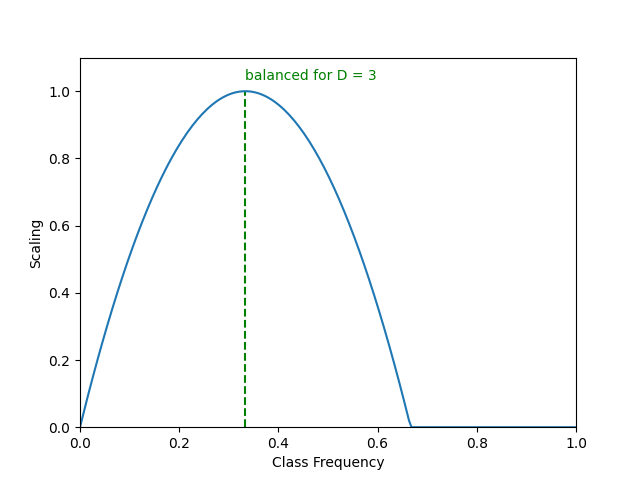
\includegraphics[width=.4\textwidth]{make_article/make_visuals/visuals/scaling.png}
    \caption{Class Frequency Scaling}
    \label{fig:scaling}
\end{wrapfigure}

\paragraph{Class Frequency Scaling.} In some cases, having a trusted user with a balanced distribution of class labels may not be possible. The ability to construct a cutoff from unbalanced data helps when data cannot be collected and avoids data privacy or security issues associated with sharing one's local class labels, or distribution thereof, with other users. From initial experimentation, we saw that either over or under-represented classes result in larger KS values for that class than benign users with a balanced distribution of class labels. Hence, we propose a simple quadratic-based scaling, see Figure \ref{fig:scaling} to scale down both over and under-represented class labels. We fit a polynomial that does not scale a balanced class and scales a class with either no representation or greater than twice the balanced frequency to zero.

\begin{algorithm}[H]
\caption{ (Class Frequency Scaling) \\ 
Notation: Let $x$ denote the vector we wish to scale and $y$ be the vector of class labels where $D$ represents the total number of unique classes for the classification problem. 
}
\label{alg:scaling}
\begin{algorithmic}[1]
    \Procedure{Class Frequency Scaling}{$\{x_c \mid c \in \mathopen[ D \mathclose] \} \mid y$}
    \State define balanced proportion for classes, $B = 1/D$
        \For{each class $c \in \mathopen[ D \mathclose]$}
            \If{class $c$ is over-represented, $x_c > 2B$}
                \State $s_c = 0$
            \Else
                \State $s_c = \dfrac{-1}{B^2}(x_c)(x_c - 2B)$
            \EndIf
        \EndFor
    \State \Return $\{s_c * x_c \mid c \in \mathopen[ D \mathclose] \}$
    \EndProcedure
\end{algorithmic}
\end{algorithm}


%
\paragraph{Global-Min Mean Smoothing. } We needed to develop a stable cutoff that is a meaningful estimate of the maximum distance a benign user can submit for a given round. We use averaging as a valuable solution for reducing variability without impacting bias. Under the assumption that certain consecutive rounds have the same values of $b_c$, we can use the average threshold across several rounds to improve our estimate's stability. Note that we can view this average as smoothing across previous values with equal weight. Although smoothing aids stability, smoothing methods tend to exacerbate the problem resulting from $b_c$ tending to decrease rapidly over the first few communication rounds. When $b_c$ decreases rapidly, we do not wish to use any previous communication rounds for our threshold as this would result in a weaker cutoff for attacks to overcome. 

Our solution is to use as our cutoff the running mean since the lowest observed value (Global-Min Mean) of the maximum class distance for the validated user. As a result, our solution quickly adapts to decreasing values of $U = max_c (b_c)$ over communication rounds. As $U$ shrinks, we are likely to observe new global minimums, and the start of the threshold is reset. In addition, when our estimate for $U$ stabilizes, the averaging smooths our cutoff, which keeps lucky malicious users from getting past a volatile threshold. 

\begin{algorithm}[H]
\caption{ (Global-Min Mean Smoothing) \\ 
Notation: Let $x$ denote the vector of values that we wish to smooth.
}
\label{alg:smoothing}
\begin{algorithmic}[1]

    \Procedure{Global-Min Mean Smoothing}{$x_n \mid x_1, \cdots, x_{n - 1}$}
        \State compute location of global minimum over communication rounds, $i = \argmin_{j: j \in \mathopen[ n \mathclose]} x_j$
        \State subset to sequence history since and including global min, $x_i^n = \{x_i, \cdots, x_n \}$
        \State \Return average of sequence subset, $\overline{x_i^n}$
    \EndProcedure
\end{algorithmic}
\end{algorithm}

We provide Figure \ref{fig:smoothing-mean} to compare our global min-mean smoothing with the base cutoff and various smoothing techniques. We believe our implementation choice best captures early behavior while providing the most remarkable improvements to stability. Additionally, when our threshold encounters a new global minimum, it provides a conservative estimate to prevent malicious users while re-learning cutoff behavior over the next few rounds.

\begin{figure}[H]
    \centering
    
    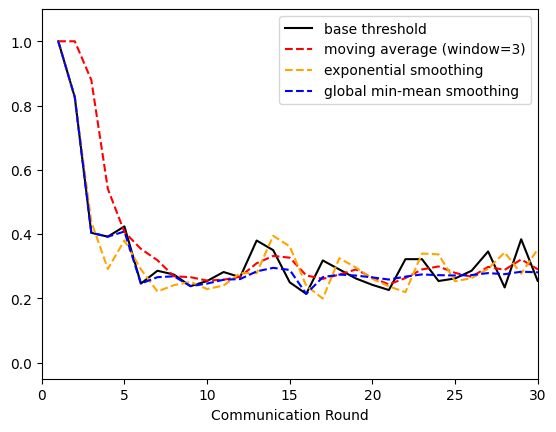
\includegraphics[width=.5\textwidth]{make_article/make_visuals/visuals/smoothing--d_rounds30.png}
    \caption{Comparison of Various Smoothing Methods}
    \label{fig:smoothing}
\end{figure}

\section{EXPERIMENTS}

%
\subsection{Setting}

\paragraph{Federated Learning.} We start by giving further specifications regarding the federated learning environment. Our interest is training a global model over M communication rounds with N users. Each iteration randomly selects K users, using a specified proportion of the total users, to participate in the model update. After local training, the next global model is the average returned model weights by the FedAvg procedure. We focus  our experiments on the ResNet18 model architecture, a standard object recognition classifier initially proposed in \cite{resnet}. 

We assume that all users, including malicious, have complete control over all aspects of local training, such as learning rate, the number of epochs, and the model weights they return. For simplicity, we select two main sets of training hyperparameters for benign and malicious users. The malicious users will poison a given proportion of their local data by adding their backdoor trigger to the input and changing the training label to that of the target class. They intend for the model to associate the trigger with the target class and hence have the future global model identify any input with the trigger as belonging to the target class. 

\paragraph{Attack.} To further show the effectiveness of our method, we choose an unrealistic and unreasonable strong attack setting. We force all malicious users to be included in the subset of users to update the global model each round after the start of the backdoor attack. Note that the selection of random users is a defense against malicious users by making it difficult for them to update the global model repeatedly. Additionally, we do not allow the validation user, a guaranteed benign user, to participate in any global model updates. We make these decisions to show the ability of our threshold to prevent even strong backdoor attacks against the global model. 


\paragraph{Data.} To produce local datasets that do not have to be independent and identically distributed, we sample from the training data set using a Dirichlet distribution with specified parameter alpha. The Dirichlet sample determines the proportion of each class included in that user's dataset. Larger values of alpha produce more balanced class distributions. We separately control alpha for benign, malicious, and validation users. Our experiments use the CIFAR-10 dataset, which consists of 60000 32x32 color images in 10 classes, with 6000 images per class. We use the test set of 10000 images, with 500 images per class, for model evaluation. 

For global model evaluation, we split the test set into two parts. We add the backdoor trigger to images in the second half and remove any target class observations. We measure model performance with classification accuracy using the first half as model success and the proportion of the poisoned half predicted as the target class, known as attack success rate, to measure the extent that the backdoor attack has compromised the model.


%
\subsection{Results}

\subsubsection{10\% Malicious}


%
\paragraph{CIFAR 10}.

\begin{figure}[H]
    \centering
    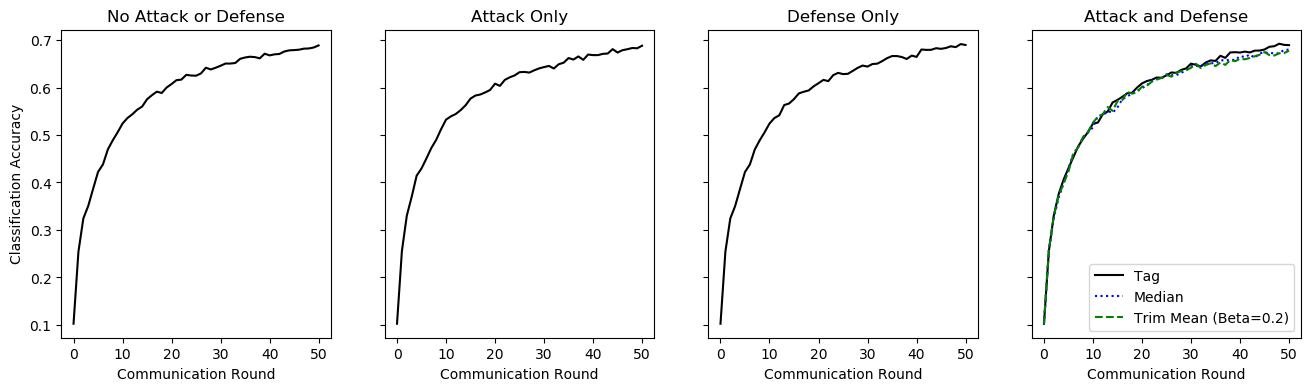
\includegraphics[width=\textwidth]{cifar_10/classic/tag/centralized/alpha10000--alpha_val10000/visuals/clean_accuracy--n_malicious1--beta0.2.png}
    \caption{Caption}
    \label{fig:my_label}
\end{figure}

\begin{figure}[H]
    \centering
    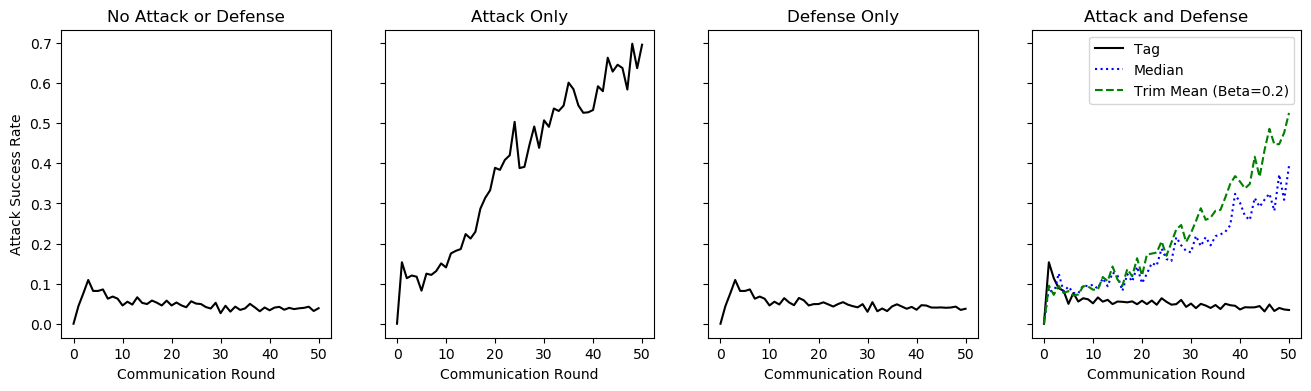
\includegraphics[width=\textwidth]{cifar_10/classic/tag/centralized/alpha10000--alpha_val10000/visuals/pois_accuracy--n_malicious1--beta0.2.png}
    \caption{Caption}
    \label{fig:my_label}
\end{figure}


%
\paragraph{CIFAR 100}.

\begin{figure}[H]
    \centering
    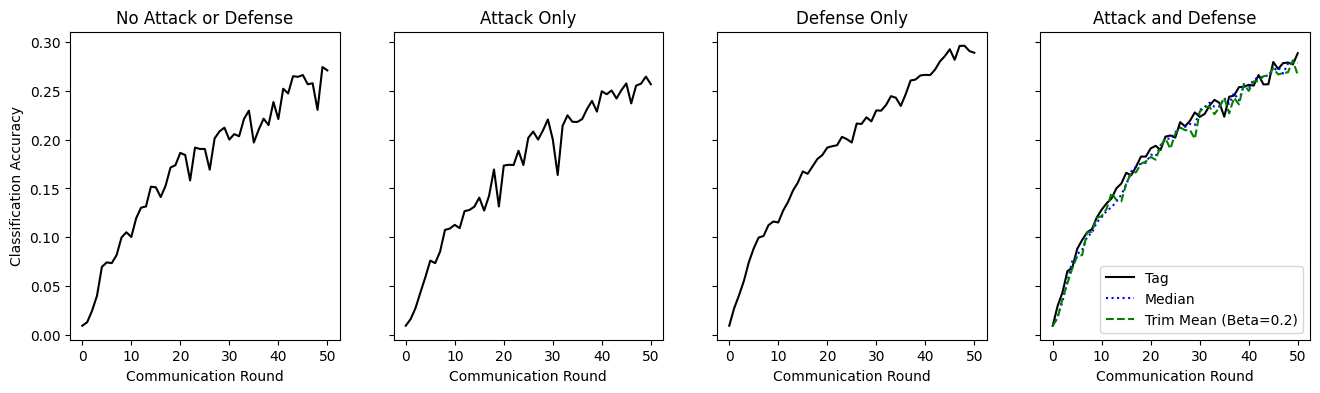
\includegraphics[width=\textwidth]{cifar_100/classic/tag/centralized/alpha10000--alpha_val10000/visuals/clean_accuracy--n_malicious1--beta0.2.png}
    \caption{Caption}
    \label{fig:my_label}
\end{figure}

\begin{figure}[H]
    \centering
    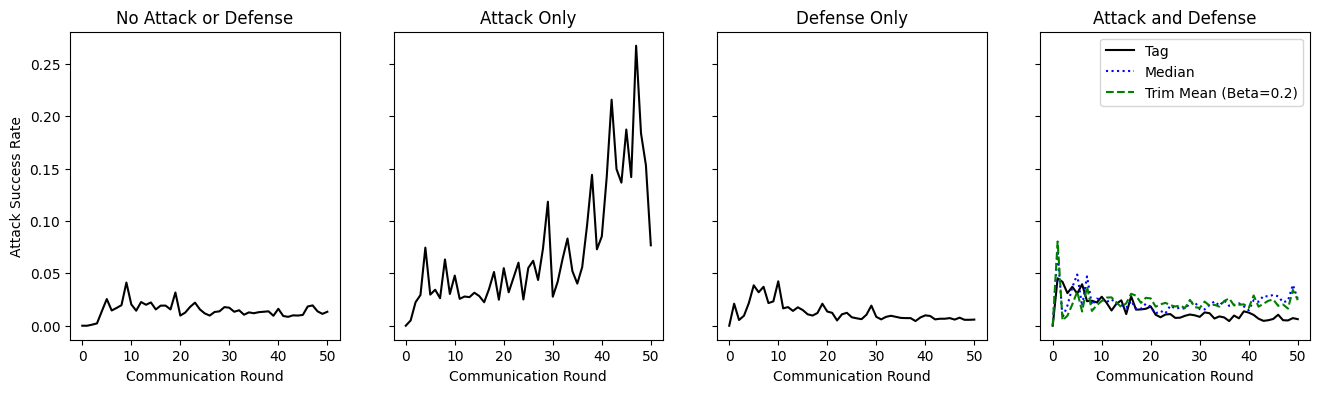
\includegraphics[width=\textwidth]{cifar_100/classic/tag/centralized/alpha10000--alpha_val10000/visuals/pois_accuracy--n_malicious1--beta0.2.png}
    \caption{Caption}
    \label{fig:my_label}
\end{figure}


%
\paragraph{STL 10}.

\begin{figure}[H]
    \centering
    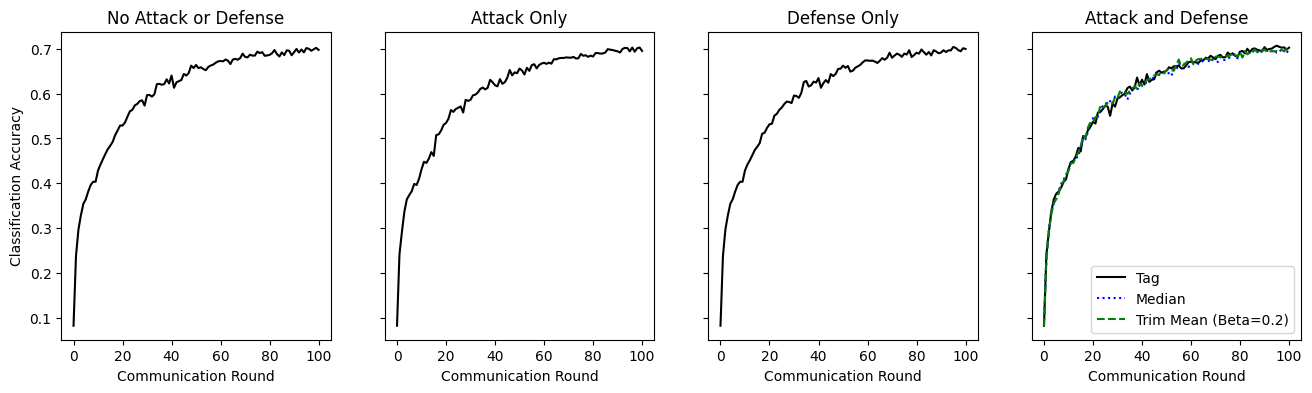
\includegraphics[width=\textwidth]{stl_10/classic/tag/centralized/alpha10000--alpha_val10000/visuals/clean_accuracy--n_malicious1--beta0.2.png}
    \caption{Caption}
    \label{fig:my_label}
\end{figure}

\begin{figure}[H]
    \centering
    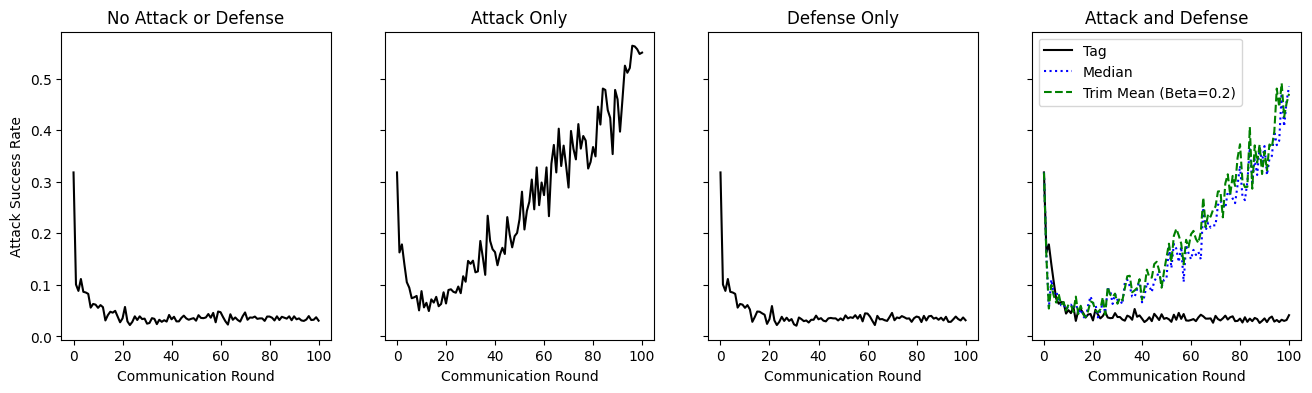
\includegraphics[width=\textwidth]{stl_10/classic/tag/centralized/alpha10000--alpha_val10000/visuals/pois_accuracy--n_malicious1--beta0.2.png}
    \caption{Caption}
    \label{fig:my_label}
\end{figure}



%
\subsection{Main Results (OLD)}

We first demonstrate the performance of our threshold when both the trusted and other users have balanced data in Figure \ref{fig:centralized--balanced--accuracy}. This figure shows the classification accuracy and the attack success rate of the global model over 250 communication rounds. For this experiment, malicious users make up 10\% of the selected users for updating the global model each round. The two leftmost figures show, without defense, that the global model can be effectively attacked where the model's classification accuracy does not change. However, the right images show that the use of our defense cutoff prevents backdoor attacks and does not decrease model performance, regardless of whether a backdoor attack is present. Furthermore, we see that the alternative aggregation methods coordinate-wise median and trimmed mean are insufficient to prevent backdoor attacks.

\begin{figure}[H]
    \centering
    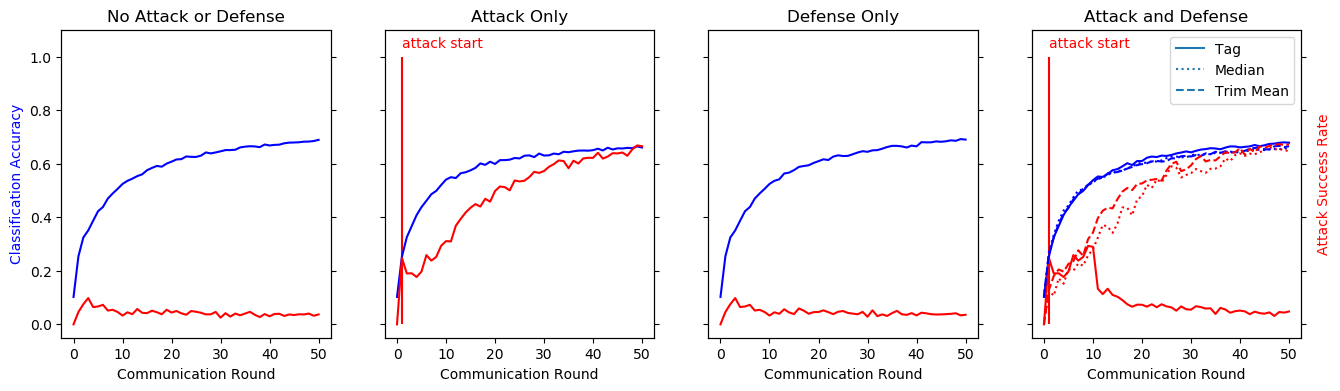
\includegraphics[width=\textwidth]{cifar_10/tag/distributed/alpha10000--alpha_val10000/visuals/accuracy--m_start1---dba1.png}
    \caption{Global Model Performance For Balanced Users And Balanced Trusted User}
    \label{fig:centralized--balanced--accuracy}
\end{figure}

Figure \ref{fig:centralized--alpha10000--alpha_val10000--threshold--n_malicious1--m_start1--d_rounds50} shows the ability of our threshold to differentiate between benign and malicious user submission. The Threshold vs. Benign figure shows the upper and lower bounds on values considered outliers for each round. We can see our threshold closely follows what we would expect to be the largest possible value a benign user contributes. Additionally, the threshold can clearly distinguish malicious users with at least one larger class output layer distributional difference. 

\begin{figure}[H]
    \centering
    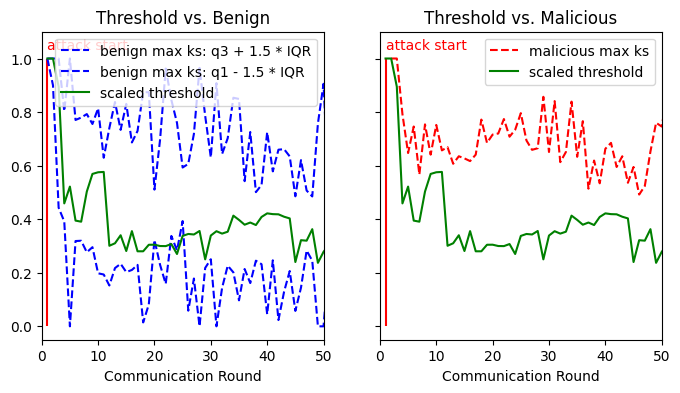
\includegraphics[width=.75\textwidth]{cifar_10/tag/centralized/alpha10000--alpha_val10000/visuals/threshold--n_malicious1--m_start1--d_rounds50.png}
    \caption{Threshold Performance For Balanced Users And Balanced Trusted User}
    \label{fig:centralized--balanced--threshold}
\end{figure}

%
\subsection{Imbalanced Data}

Next, we highlight the ability of our threshold to estimate these benign users' upper bound even when the validation user has imbalanced data. As shown in Figure \ref{fig:centralized--alpha10000--alpha_val1--scaling--d_rounds50.png}, the scaled threshold corrects for the large Kolmogorov Smirnov values of imbalanced classes and gives a reasonable representation for the most considerable value that a benign user with balanced data. The model and threshold performance remain similar to the balanced validation user case; see Appendix \ref{sec.imbal_val} for actual plots. Scaling is necessary to reduce the enormous opportunity of malicious users to backdoor the global model in the early communication rounds.

\begin{figure}[H]
    \centering
    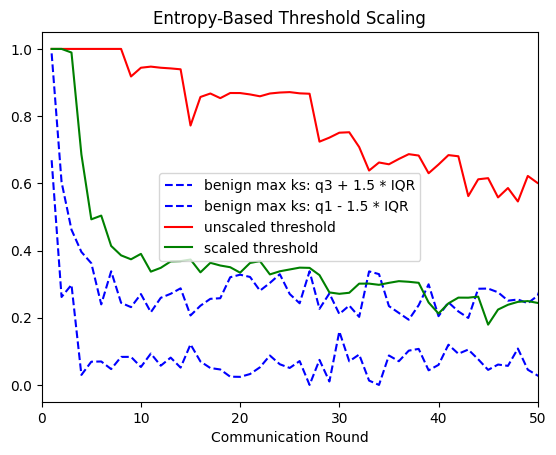
\includegraphics[width=.5\textwidth]{01_trusted/centralized/alpha10000--alpha_val1/visuals/scaling--n_malicious1--m_start1--d_rounds50.png}
    \caption{Caption}
    \label{fig:centralized--alpha10000--alpha_val1--scaling--d_rounds50.png}
\end{figure}

Our threshold is also effective against backdoor attacks when the users have imbalanced data. See Appendix \ref{sec.imbal_users} for model performance plots under this setting. Recall our earlier observation that imbalanced data is associated with more considerable class differences between the global and returning models. Therefore, in this case, the benign users will return models that fail to pass our threshold more often. Note that our threshold should not be modified for this setting as a malicious user with balanced data would have an easier time performing a backdoor attack on the global model. In summary, attempting to train a backdoor-free robust model will take additional training time when users have imbalanced data.

\subsection{Distributed Backdoor Attacks (DBA)}

We now focus on highlighting our threshold's performance under an unrealistically strong attack setting. Here we consider multiple attackers that makeup 40\% of the subset of users to update the global model every communication round. Furthermore, the backdoor trigger has been geometrically distributed between the attackers using the Distributed Backdoor Attack procedure defined in \cite{dba}. In Figure \ref{fig:distributed--alpha10000--alpha_val10000--accuracy}

\begin{figure}[H]
    \centering
    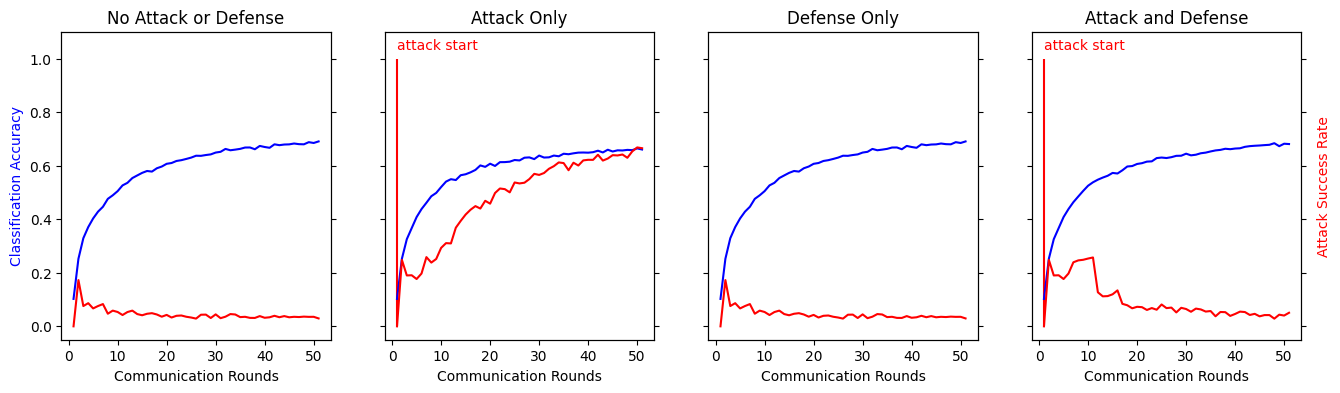
\includegraphics[width=\textwidth]{01_trusted/distributed/alpha10000--alpha_val10000/visuals/accuracy--n_malicious4--m_start1.png}
    \caption{Caption}
    \label{fig:distributed--alpha10000--alpha_val10000--accuracy}
\end{figure}

Threshold struggles with many attackers and strongly imbalanced user data - less benign updates.

% 
\section{Conclusion}

%
\bibliography{iclr2023_conference}
\bibliographystyle{iclr2023_conference}

%
\appendix

%
\section{Main Results Continued}

%
\subsection{Balanced Users, Imbalanced Validation User}
\label{sec.imbal_val}

\begin{figure}[H]
    \centering
    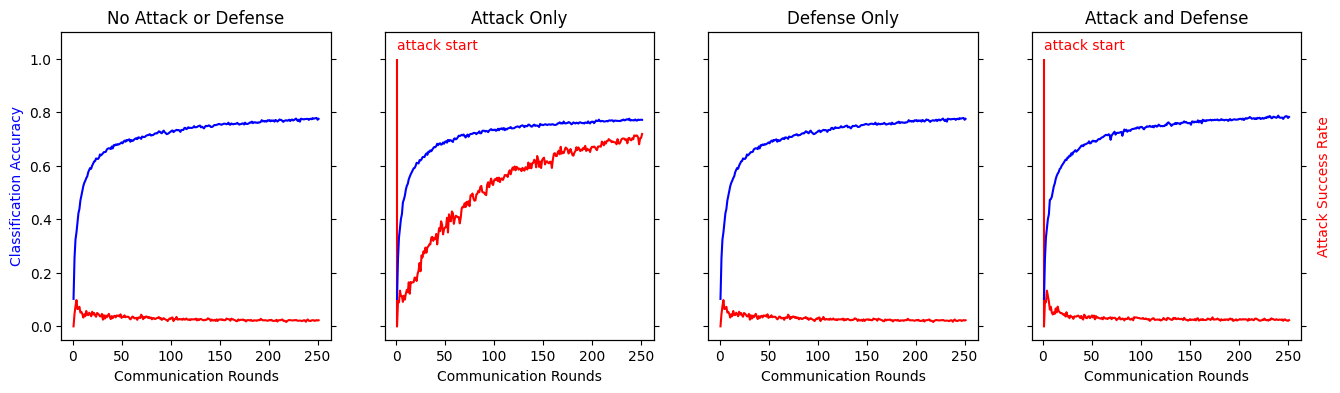
\includegraphics[width=\textwidth]{01_trusted/centralized/alpha10000--alpha_val1/visuals/accuracy--n_malicious1--m_start1.png}
    \caption{Global Model Performance For Balanced Users And Imbalanced Trusted User}
    \label{fig:centralized--alpha10000--alpha_val1--accuracy--n_malicious1--m_start1}
\end{figure}

\begin{figure}[H]
    \centering
    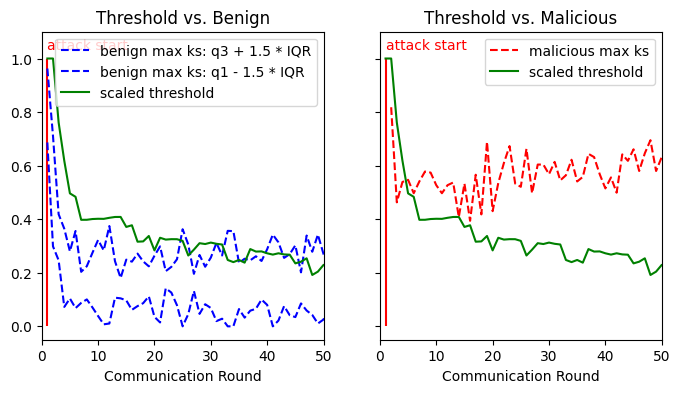
\includegraphics[width=.75\textwidth]{01_trusted/centralized/alpha10000--alpha_val1/visuals/threshold--n_malicious1--m_start1--d_rounds50.png}
    \caption{Threshold Performance For Balanced Users And Imbalanced Trusted User}
    \label{fig:centralized--alpha10000--alpha_val1--threshold--n_malicious1--m_start1--d_rounds50}
\end{figure}

%
\subsection{Balanced Users, Imbalanced Validation User}
\label{sec.imbal_users}

\begin{figure}[H]
    \centering
    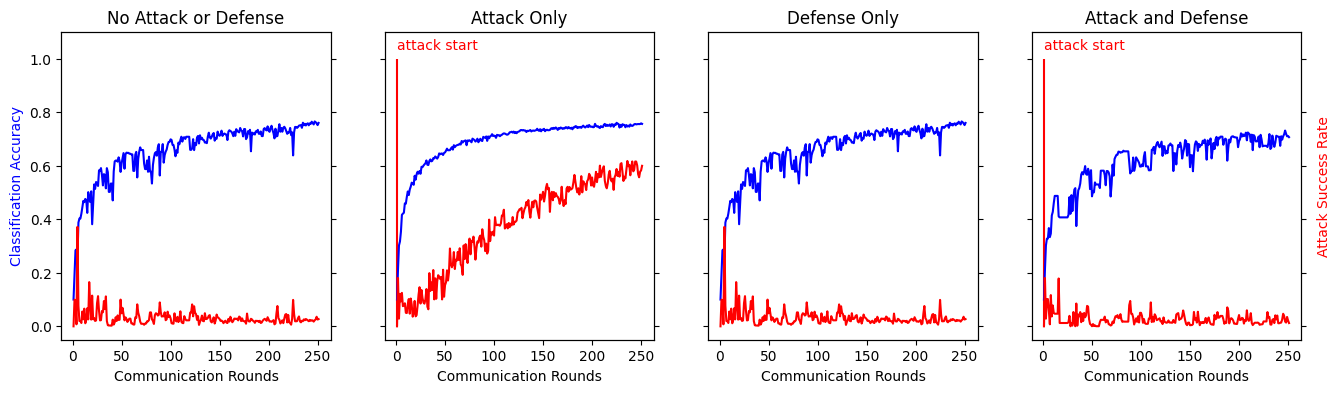
\includegraphics[width=\textwidth]{01_trusted/centralized/alpha1--alpha_val1/visuals/accuracy--n_malicious1--m_start1.png}
    \caption{Global Model Performance For Imbalanced Users And Balanced Trusted User}
    \label{fig:centralized--alpha1--alpha_val10000--accuracy--n_malicious1--m_start1}
\end{figure} 

\begin{figure}[H]
    \centering
    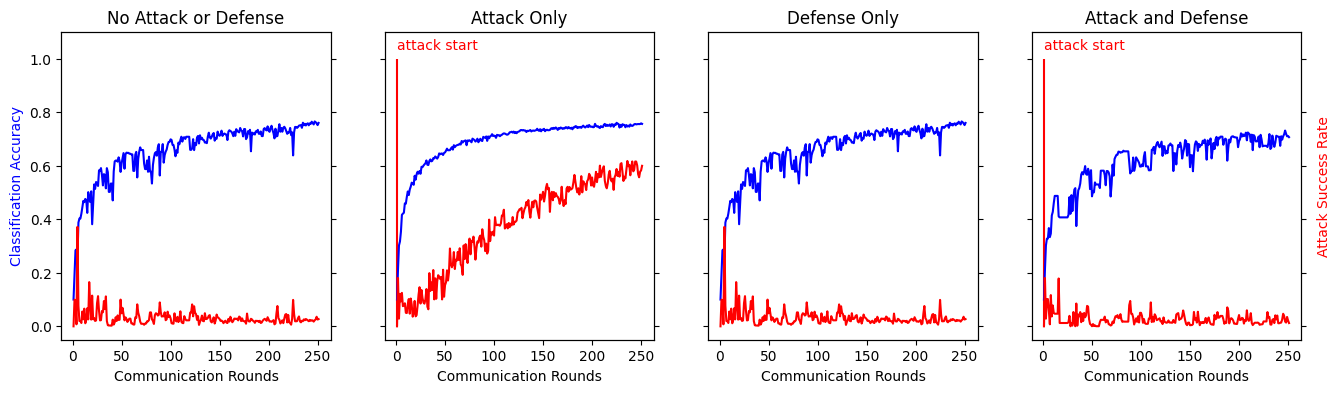
\includegraphics[width=\textwidth]{01_trusted/centralized/alpha1--alpha_val1/visuals/accuracy--n_malicious1--m_start1.png}
    \caption{Global Model Performance For Imbalanced Users And Imbalanced Trusted User}
    \label{fig:centralized--alpha1--alpha_val1--accuracy--n_malicious1--m_start1}
\end{figure} 



% 
\section{Retired Text (Saved If Needed Later)}

%
\subsection{Warm-up Period}

Our final threshold includes a warm-up period, global min-mean smoothing, and class frequency scaling to address the above concerns, respectively.

If we make the additional assumption of independence between classes distributions, we can show, see Equation \ref{eq:leq_bound} that alternative scaling of the maximum distance can instead produce a estimator that is conservative, on average. Furthermore, Equation \ref{eq:leq_bound} holds with equality instead when class distances share identical supports (ie. $\forall c \in \mathopen[ D \mathclose], b_c = b$). Note that the conservative scaling $(D + 1) / D \in \mathopen(1, \mathclose 1.5]$, and that larger classification problems require smaller initial scaling. This agrees with intuition that larger-way classification problems may require longer warm-up periods. 

\begin{align}
    & \textrm{Suppose } \forall c \in \mathopen[ D \mathclose], (KS)_c \overset{\indep}{\sim} Uniform(0, b_c) \nonumber \\
    & \quad \dfrac{(KS)_c}{b_c} \overset{\mathrm{iid}}{\sim} Uniform(0, 1) \nonumber \\
    & \quad \max_c \left( \dfrac{(KS)_c}{b_c} \right) \sim Beta(D, 1) \nonumber \\
    & \textrm{Let } j = \argmax_c \left( b_c \right) \textrm{ such that } b_j = \max_c \left( b_c \right) \nonumber \\
    & \quad \max_c \left( \dfrac{(KS)_c}{b_j} \right) \leq \max_c \left( \dfrac{(KS)_c}{b_c} \right) \nonumber \\
    & \quad E \left[ \max_c \left( \dfrac{(KS)_c}{b_j} \right) \right] \leq E \left[ \max_c \left( \dfrac{(KS)_c}{b_c} \right) \right] = \dfrac{D}{D + 1} \nonumber \\
    & \quad E \left[ \left( \dfrac{D + 1}{D} \right) \max_c \left( (KS)_c \right) \right] \leq b_j \label{eq:leq_bound}
\end{align}

We recommend traversing coefficients from $(D + 1) / D$ to 2 to assist in dampening the large opportunity for malicious users to impact the global model at the beginning of Federated Learning. It may be often more practical, additional training time permitting, to start with scaling by 1 to avoid fine-tuning this procedure for large classification problems. Additionally, we believe that the length and intermediate values chosen, should be greatly influenced by the context of the application. Longer warm-up periods may be most useful when there is greater chance or consequence of attack.


\subsection{Computation}
Only the validation user's local training, requiring gradient calculations, is an additional step with a high relative computational cost. However, users often train on local compute resources in the Federated Learning setting. Therefore, the validation user will do this step simultaneously with the local training of other users, largely avoiding extra training time. The only other steps not already done during Federated Learning are forward passes, which are less complex and quickly accelerated by modern computing architectures. \yli{We can discuss the advantage of the method at the end of sec 3. Let's focus on describing the method first.}

We make use of the empirical CDF function to avoid distributional assumptions on the output layers and KS distances for computational efficiency. Using the property that the empirical CDFs are step functions, note that the KS distance between the empirical CDFs only needs to be computed for each of the values of the class scores on the local user's data for both the global and trusted user's updated model, which is easily computed in-parallel.

%
\subsection{Entropy-Based Scaling}
From information theory, Shannon Entropy is one such measure of diversity. Note that entropy is maximized when class labels are uniformly distributed. 

We propose scaling the KS distances between global and updated models for each class $(KS)_c$ by the following factor $S_c$, before computing the maximum and multiplying by two. Note that $S$, the collection of $S_c$, only needs to be computed once, as it depends on the local user's class label distribution and does not depend on the distance values each round.

\begin{definition}[Shannon Entropy] For a discrete random variable Y, taking values $v$, with probability mass function $p(y)$, Shannon Entropy is defined as $H(Y) = - \sum_{v} p(v) \log p(v)$.
    
\end{definition}

\begin{align}
    y_c &= \min \left( x_c, \dfrac{1}{e} \right) \\
    z_c &= \min \left( \dfrac{P(y_c) \ln \left( P(y_c) \right)}{\dfrac{1}{D} \ln \left( \dfrac{1}{D} \right)}, 2 \right) \\
    S_c &= 1 - | 1 - z_c |    
\end{align}

% figure omitted
See Figure \ref{fig:scaling} for $S_c(x)$ plotted as a function of the class proportions for several values of $D$, the total number of classes. Observe the following  properties:
\begin{enumerate}
    \item Scaling is between 0 and 1, and there is no scaling when a given class is balanced
    \item Under-represented classes are scaled down to zero
    \item For many-class classification problems, we are less trusting of an over-represented class as we have more potential classes for at least one to be approximately balanced.
\end{enumerate}

We believe further research is needed regarding extremely imbalanced edge cases. However, we propose this scaling as a remedy for reasonably imbalanced data, demonstrating its promising effectiveness in our experimentation.


\end{document}
